\documentclass[a4paper]{article}

\usepackage[width=14cm, left=3cm, top=3cm]{geometry}

\usepackage[brazil]{babel}
\usepackage[T1]{fontenc}
\usepackage[utf8]{inputenc}

\usepackage{hyperref}

\usepackage{graphicx}

\usepackage{amsmath}
\usepackage{amssymb}

% No indent
\setlength{\parindent}{0pt}
\setlength{\parskip}{2ex}

\newcommand{\linkfileraw}[2]{\href{run:../../#1}{\texttt{#2}}}
\newcommand{\linkfile}[2][src/05-finite-elements-gamma/]{\linkfileraw{#1#2}{#2}}

\newcommand{\typ}{\::\:}

\newcommand{\vphi}{\varphi}

\title{Trabalho 01 --- Elementos Finitos}
\author{Daniel Kiyoshi Hashimoto Vouzella de Andrade -- 124259224}
\date{24 de Setembro de 2024}

\begin{document}
\maketitle

\setcounter{section}{-1}
\section{Implementação}

A implementação (e esse pdf) está em
\href{https://github.com/Kiyoshi364/finite-elements}{github.com/Kiyoshi364/finite-elements}.
O pdf está sendo feio em cima do commit
\texttt{365e28bbdca537e48f6eb6afc77e6756017df39a},
então o commit de entrega deve ser o seguinte a esse.

A implementação está na pasta
\linkfileraw{/src/05-finite-elements-gamma/}{/src/05-finite-elements-gamma/},
(os outros arquivos serão indicados
relativamente a essa pasta).
O arquivo \linkfile{finite-elements.jl}
é ``a biblioteca'',
enquanto
\linkfile{solution.jl} e \linkfile{errors.jl}
são os ``scripts'' que rodam os experimentos pedidos
e geram as imagens incluídas no final do pdf\footnote{
Para que os scripts gerem uma imagem,
é necessário alterar o nome do arquivo de saída
em cada script para ter uma extensão de imagem
(ou não ter extensão nenhuma).
Por padrão eles geram um pdf.
}.
Para que os exemplos que os scripts rodam
sejam o mesmo do pedido
(\(u(x) = \sin(\pi \; x)\)),
escolha o exemplo \(0x3\)
no início dos scripts.
O exemplo está definido
no arquivo
\linkfile{../examples.jl}
na função \texttt{bacarmo\_example\_gamma}.
Outro arquivo usado pela biblioteca é
\linkfile{../common.jl}
que possui algumas funções e códigos auxiliares,
como cálculo de erro e
tabela de pontos e pesos da quadratura de Gauss.

\section{Formulação Forte}

Dados
\(f \typ [0, 1] \to \mathbb{R}\),
\(\alpha > 0\),
\(\beta \ge 0\),
\(\gamma \ge 0\),
o objetivo é descobrir \(u \typ [0, 1] \to \mathbb{R}\)
que satisfaça o sistema:
\[
    \begin{cases}
        - \alpha \; u_{xx}(x) + \beta \; u(x) + \gamma \; u_{x}(x) = f(x)
            \quad\text{, } x \in (0, 1) \\
        u(0) = u(1) = 0
    \end{cases}
\]

\section{Transição entre Forte e Fraca}

Sejam o espaço das soluções:
\[
    H = \{
        u \text{ é suficientemente suave } : u(0) = u(1) = 0
    \}
\]
e o espaço das funções de teste (funções peso)
\[
    V = \{
        v \text{ é suficientemente suave } : v(0) = v(1) = 0
    \}
\]

\emph{Nota}: Nesse caso \(H = V\).

Seja \(v \in V\) qualquer,
simplificamos (enfraquecemos) o problema inicial:
\[
    - \alpha \; \int_0^1{ u_{xx}(x) \; v(x) \; dx }
    + \beta \; \int_0^1{ u(x) \; v(x) \; dx }
    + \gamma \; \int_0^1{ u_x(x) \; v(x) \; dx}
    = \int_0^1{ f(x) \; v(x) \; dx }
\] \[
    - \alpha \; \left[ \left( v(x) \; u_x(x) \right|_0^1 - \int_0^1{ u_x(x) \; v_x(x) \; dx } \right]
    + \beta \; \int_0^1{ u(x) \; v(x) \; dx }
    + \gamma \; \int_0^1{ u_x(x) \; v(x) \; dx}
    = \int_0^1{ f(x) \; v(x) \; dx }
\] \[
    - \alpha \; \left[ - \int_0^1{ u_x(x) \; v_x(x) \; dx } \right]
    + \beta \; \int_0^1{ u(x) \; v(x) \; dx }
    + \gamma \; \int_0^1{ u_x(x) \; v(x) \; dx}
    = \int_0^1{ f(x) \; v(x) \; dx }
\] \[
    \alpha \; \int_0^1{ u_x(x) \; v_x(x) \; dx }
    + \beta \; \int_0^1{ u(x) \; v(x) \; dx }
    + \gamma \; \int_0^1{ u_x(x) \; v(x) \; dx}
    = \int_0^1{ f(x) \; v(x) \; dx }
\]

Juntando tudo:
\[ \begin{cases}
    \alpha \; \int_0^1{ u_x(x) \; v_x(x) \; dx }
    + \beta \; \int_0^1{ u(x) \; v(x) \; dx }
    + \gamma \; \int_0^1{ u_x(x) \; v(x) \; dx}
    = \int_0^1{ f(x) \; v(x) \; dx } \\
    u(0) = u(1) = 0 \\
    v(0) = v(1) = 0
\end{cases} \]

\section{Formulação Fraca}

Dados
\(f \typ [0, 1] \to \mathbb{R}\),
\(\alpha > 0\),
\(\beta \ge 0\),
\(\gamma \ge 0\),
o objetivo é descobrir \(u \in H\)
que para qualquer \(v \in V\),
satisfaça a equação:
\[
    \alpha \; \int_0^1{ u_x(x) \; v_x(x) \; dx }
    + \beta \; \int_0^1{ u(x) \; v(x) \; dx }
    + \gamma \; \int_0^1{ u_x(x) \; v(x) \; dx}
    = \int_0^1{ f(x) \; v(x) \; dx }
\]

Usando uma notação extra:
\begin{itemize}
\item \[
    \kappa(u, v) =
    \alpha \; \int_0^1{ u_x(x) \; v_x(x) \; dx }
    + \beta \; \int_0^1{ u(x) \; v(x) \; dx }
    + \gamma \; \int_0^1{ u_x(x) \; v(x) \; dx}
\]
\item \[
    (u, v) =
    \int_0^1{ u(x) \; v(x) \; dx }
\]
\end{itemize}
conseguimos ``simplificar'' a equação:
\[
    \kappa(u, v) = (f, v)
\]

\section{Problema Aproximado via o Método de Galerkin}

Seja o espaço das soluções
\[
    H^h = \{
        u \text{ é suficientemente suave } : u(0) = u(1) = 0
    \}
\]
e o espaço das funções de teste (funções peso)
\[
    V^h = \{
        v \text{ é suficientemente suave } : v(0) = v(1) = 0
    \}
\]
ambos tendo dimensão finita \(m\)
e base \(\{ \vphi_1, \vphi_2, \dots, \vphi_m\}\).

\emph{Nota}: Nesse caso \(H^h = V^h\).

Dados
\(f \typ [0, 1] \to \mathbb{R}\),
\(\alpha > 0\),
\(\beta \ge 0\),
\(\gamma \ge 0\),
o objetivo é descobrir \(u_h \in H^h\)
que para qualquer \(v_h \in V_m\),
satisfaça a equação:
\[
    \kappa(u^h, v^h) = (f, v^h) \\
\]

\section{Transição entre Problema Aproximado e Forma Matriz-Vetor}

Como estamos trabalhando em um espaço discreto,
podemos descrever \(u^h\)
como uma ``soma pesada'' dos elementos da base:
\[
    u^h = \sum_{j=1}^m{ c_j \; \vphi_j }
\]


Como os \(\vphi_1, \dots, \vphi_m\)
são uma base do espaço \(V_m\),
é suficiente satisfazer o sistema
apenas para os elementos da base.

Juntando as duas informações,
criamos um sistema de \(m\) linhas.
Cada linha do sistema tem a seguinte forma,
com \(i = 1, \dots, m\):
\[
    \kappa(\sum_{j=1}^m{ c_j \; \vphi_j }, \vphi_i) = (f, \vphi_i)
\] \[
    \sum_{j=1}^m{ \kappa(c_j \; \vphi_j, \vphi_i) } = (f, \vphi_i)
\] \[
    \sum_{j=1}^m{ c_j \; \kappa(\vphi_j, \vphi_i) } = (f, \vphi_i)
\]

Abrindo o \(\sum\), temos uma linha da forma:
\[
    c_1 \; \kappa(\vphi_1, \vphi_i)
    + c_2 \; \kappa(\vphi_2, \vphi_i)
    + \cdots
    + c_m \; \kappa(\vphi_m, \vphi_i)
    = (f, \vphi_i)
\]

\section{Forma Matriz-Vetor}

Dados
\(f \typ [0, 1] \to \mathbb{R}\),
\(\alpha > 0\),
\(\beta \ge 0\),
\(\gamma \ge 0\),
o objetivo é descobrir os coeficientes \(c_j\)
de \(c\)
satisfaçam a equação matricial:
\[
    \mathbb{K} \; c = \mathbb{F}
\]
onde:
\begin{itemize}
\item \[
    \mathbb{K}_{i, j} = \kappa(\vphi_j, \vphi_i)
\]
\item \[
    \mathbb{F}_i = (f, \vphi_i)
\]
\end{itemize}

\section{Resultados}

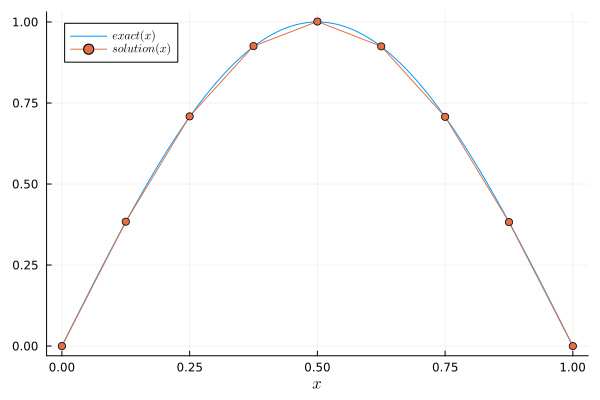
\includegraphics[width=0.5\textwidth]{images/solucao_aprox}
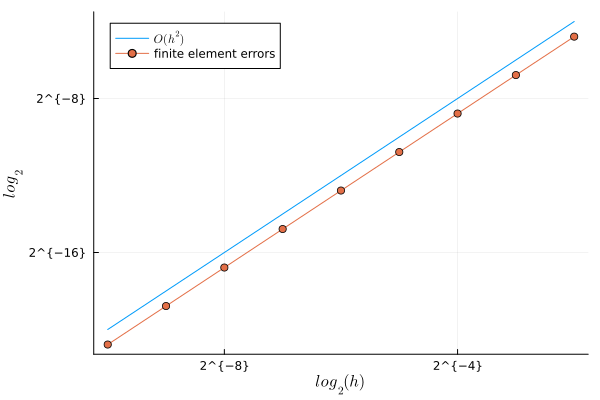
\includegraphics[width=0.5\textwidth]{images/convergencia_erro}

\end{document}
